%% Vaaraible independiente Deep Learning Visión por computadora


\subsection{Inteligencia Artificial}
La inteligencia artificial (IA) se enfoca en crear sistemas y programas capaces de realizar tareas de la misma manera que lo haría un ser humano. Estos sistemas están diseñados para adaptarse y mejorar con la experiencia, reconocer patrones, tomar decisiones y aprender de datos. 

El termino Inteligencia Artificial fue dado a conocer en el año 1956 durante la Conferencia Dartmouth en Hanover, Nuevo Hampshire (Estados Unidos), donde se propuso la posibilidad de crear una máquina que pudiera pensar como un ser humano.  No obstante, esta a estado presente mucho antes desde de trabajos de investigación, hasta en el cine y novelas representando como ciencia ficción. 
Actualmente, se ha convertido en una de las tecnologías revolucionarias y de mayor interés de investigación.


\begin{figure}[h]
	\begin{center}
		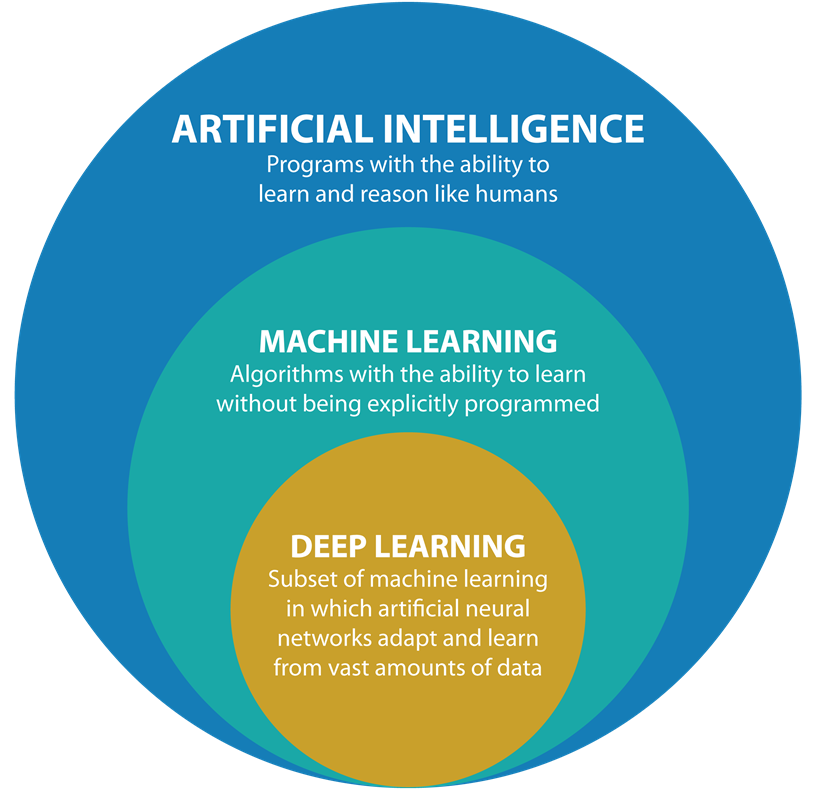
\includegraphics[width=0.5\textwidth]{2/figuras/imagenes/IA_ML_DL.png}
		\caption{Grafico de IA. Fuente: \cite{IA_}}
		\label{1:fig 16}
	\end{center}
\end{figure}

\subsection{Features Vectors}
Un vector de características, es una representación numérica de un objeto, instancia o dato en un espacio multidimensional, donde cada dimensión del vector corresponde a una característica particular del objeto. Estos vectores se utilizan en una variedad de campos, especialmente en el Machine Learning(ML) y Deep Learning(DL), para hacer predicciones y entrenar modelos.

Son cruciales porque pueden capturar de manera efectiva las propiedades pertinentes de los datos, lo que facilita el aprendizaje de los modelos y mejora su rendimiento predictivo. Un buen diseño puede aumentar la velocidad de entrenamiento y reducir la complejidad de los problemas.


\subsubsection{GLCM (Gray Level Co-occurrence Matrix)}

La Matriz de Co-ocurrencia de Niveles de Gris (GLCM), también denominada matriz de dependencia espacial de escala de gris, es una herramienta utilizada en el campo de la visión por computadora y el procesamiento de imágenes para analizar la textura de una imagen. Este captura la relación espacial entre los píxeles en una imagen al cuantificar la frecuencia con la que pares de valores de intensidad de píxeles ocurren juntos en diferentes direcciones y distancias. Este método estadístico para analizar la textura toma en cuenta la relación espacial de los píxeles, creando una GLCM y extrayendo medidas estadísticas de esta matriz. Las funciones de GLCM caracterizan la textura de una imagen calculando con qué frecuencia los pares de píxeles que muestran valores específicos y se encuentran en una relación espacial concreta ocurren en una imagen. Una vez creadas las GLCM usando graycomatrix, se pueden derivar varias estadísticas de ellas empleando graycoprops, proporcionando información detallada sobre la textura de la imagen.
\parencite{mathworksAnxE1lisisTextura}

\subsubsection{Moment Invariant}

Los Momentos Invariantes son características numéricas de una distribución de píxeles en una imagen que son invariantes a transformaciones geométricas como traslación, rotación y escala. Estos momentos, calculados a partir de los valores de intensidad de los píxeles, estos momentos proporcionan información sobre la forma y la distribución de los objetos en la imagen. Se utilizan en aplicaciones como el reconocimiento de formas, describiendo la forma de objetos en imágenes para identificar y reconocer patrones independientemente de su orientación o tamaño, y en la detección de objetos, donde sirven como características para detectar objetos en imágenes basándose en su forma y estructura.


\subsubsection{GLRLM (Gray Level Run Length Matrix)}
La Matriz de Longitud de Corrida de Niveles de Gris (GLRLM) es una técnica utilizada para analizar la textura de una imagen midiendo la longitud y la frecuencia de regiones contiguas con el mismo nivel de gris en diferentes direcciones. Esta técnica describe cuántas veces aparecen píxeles con un cierto nivel de gris en una imagen a lo largo de una dirección específica, proporcionando información sobre la homogeneidad y la textura de la imagen. La GLRLM se calcula para diferentes direcciones, generalmente 13 en 3D o 4 en 2D, y para cada nivel de gris, la matriz contiene la cantidad de veces que aparece una secuencia continua de píxeles con ese nivel de gris en una dirección específica.

Se utiliza en diversas aplicaciones, como el análisis de imágenes médicas, el procesamiento de imágenes industriales, la segmentación de texturas y el reconocimiento facial. La GLRLM permite extraer características de textura como la longitud promedio de carrera, la intensidad promedio y la homogeneidad, y ayuda a identificar regiones inusuales o anómalas en una imagen al detectar patrones de textura distintivos.


\subsection{Aprendizaje Automático  (Maching Learning)}
Es un subcampo de la inteligencia artificial que se centra en el desarrollo de algoritmos y modelos. Permitiendo a las computadoras aprender a partir de datos ya etiquetados y tomar decisiones según la información brindada, esto identificando patrones en los datos y utilizando estos para hacer predicciones o tomar decisiones.
Este tiende a aplicarse en los siguientes temas: detección de fraudes, predicciones, clasificación, sistemas de recomendación.
Este aprendizaje requiere datos de entrenamiento para que funcionen, ademas de mayormente trabajar con data estructurada.

\subsubsection{K-Nearest Neighbors (KNN)}
El algoritmo de K-Nearest Neighbors (KNN) es un método de aprendizaje supervisado utilizado tanto para problemas de clasificación como de regresión. Funciona asignando una etiqueta de clase a un punto de datos basándose en la mayoría de las etiquetas de clase de sus vecinos más cercanos en el espacio de características. En otras palabras, clasifica un punto de datos basándose en las clases de los puntos que están más cerca de él en el espacio de características.

El funcionamiento del algoritmo KNN es relativamente simple: dado un nuevo punto de datos, el algoritmo calcula la distancia entre ese punto y todos los demás puntos de datos en el conjunto de entrenamiento. Luego, selecciona los K puntos más cercanos (vecinos) al nuevo punto y determina la clase mayoritaria entre estos vecinos. Esa clase mayoritaria se asigna al nuevo punto de datos como su etiqueta de clase. La elección del valor de K es crítica y puede afectar significativamente el rendimiento del algoritmo: valores más pequeños de K pueden hacer que el modelo sea más susceptible al ruido, mientras que valores más grandes de K pueden dar como resultado fronteras de decisión más suaves pero también pueden disminuir la precisión del modelo. KNN es un algoritmo simple pero poderoso, especialmente para conjuntos de datos pequeños o cuando no se asume una estructura particular en los datos. Sin embargo, su eficacia puede verse limitada en conjuntos de datos con muchas características o cuando los datos están altamente dimensionales.


%\subsubsection{Random Forest (RF)}

%\subsubsection{Decision Tree}

%\subsubsection{XGBoost}

%\subsubsection{Probabilistic Neural Network (PNN)}

\subsection{Aprendizaje Profundo (Deep Learning)}
Es un subcampo del aprendizaje automático que utiliza redes neuronales artificiales con múltiples capas (profundas) para modelar y resolver problemas complejos. Las redes neuronales profundas se caracterisan por la necesidad de recibir grandes conjuntos de datos estos pueden ser estructurados o no estructurado. Con la finalidad de aprender representaciones jerárquicas de los datos, lo que permite la automatización de la extracción de características.

Este tiende a aplicarse en los siguientes temas: Reconocimiento de voz y visión por computadora, procesamiento de lenguaje natural (NLP), Diagnóstico médico, conducción autónoma, entre otros.

%\subsubsection{EfficientNets}

\subsubsection{Deep Neural Networks (DNN)}
Son modelos de aprendizaje automático que se destacan por su estructura de múltiples capas de neuronas, permitiendo aprender representaciones complejas de los datos. Estas redes están diseñadas para realizar un aprendizaje jerárquico, donde las primeras capas aprenden características simples de los datos de entrada, mientras que las capas posteriores combinan estas características para formar representaciones más abstractas y sofisticadas.

El funcionamiento implica procesar los datos de entrada a través de varias capas de neuronas y ajustar los pesos de la red iterablemente mediante retropropagación del error para reducir las diferencias entre los resultados reales y las predicciones del modelo. Este método de aprendizaje profundo ha demostrado un gran éxito en una variedad de campos, como la robótica, el procesamiento de lenguaje natural y la visión por computadora, ofreciendo soluciones poderosas y automatizadas para una amplia gama de problemas de análisis de datos y toma de decisiones.




%\subsubsection{Deep Convolutional Neural Network (DCNN)}




\subsection{Computer Vision}
Se centra en entrenar a las máquinas para que interpreten las imágenes o videos de manera similar a como lo hacen los humanos. Esto implica la adquisición, el procesamiento, el análisis y la comprensión de imágenes y datos visuales para automatizar tareas que requieren la visión humana.
Algunas tecnologías y algoritmos en esta área son:
\newcommand{\CVone}{ Comparación estadística: Los algoritmos son capaces de  realizar comparaciones y análisis detallados de los objetos, más allá de ubicarlos en un plano.}
\newcommand{\CVtwo}{Detección de objetos: Los algoritmos son capaces de localizar y claisficar varios objetos en una imagen o en videos. Algunos algoritmos son YOLO (You Only Look Once), SSD (Single Shot MultiBox Detector), Faster R-CNN }
\newcommand{\CVthree}{ Análisis de Movimiento: Capacidad de seguir el movimiento y la dirección de un objetos o personas en una secuencia de video. Ejemplos: Optical Flow, Tracking algorithms (Kalman Filter, Mean-Shift, etc.). }

\begin{itemize}
	\item \CVone
	\item \CVtwo
	\item \CVthree
\end{itemize}
